\documentclass[spanish]{beamer}
\usepackage[utf8]{inputenc}
\usepackage{float}
\usepackage{beamerthemesplit}
\usepackage{latexsym}
\usepackage[T1]{fontenc}
\usepackage{amsmath}
\usepackage{hyperref}
\usepackage{graphicx}
\usepackage{babel,blindtext}
\usepackage{amsfonts}
\usepackage[round]{natbib}
\bibliographystyle{chicago}
\usepackage{subcaption} 


\decimalpoint

\usetheme{Antibes}%este es el templete que se usa a lo largo de la presentacion
%themes
%   default
%   Boadilla
%   Madrid
%   Pittsburgh
%   Copenhagen
%   Warsaw
%   Singapore
%   Malmoe
\newcommand\Fontvi{\fontsize{6}{7.2}\selectfont}
\mode<presentation>%tipo de 
\begin{document}

%%%%%%%%%%%%%%%%%%%%%%%%%%%%%%%%%%%%%%%%%%%%%%%%%%%%%%%%%%%%%%%%%%%%%%%%%%%%%%%%%%%%%%%%%%%%%%%%%%%%%%%%%%%%%
\title{Poisson Processes}
\author{Gamaliel Moreno Chávez}
\institute{MCPI}
\date{Ago-Dic\\ 2020}%para que ponga la fecha de hoy 

\frame{\titlepage}
%%%%%%%%%%%%%%%%%%%%%%%%%%%%%%%%%%%%%%%%%%%%%%%%%%%%%%%%%%%%%%%%%%%%%%%%%%%%%%%%%%%%%%%%%%%%%%%%%%%%%%%%%%%%%
%%%%%%%%%%%%%%%%%%%%%%%%%%%%%%%%%%%%%%%%%%%%%%%%%%%%%%%%%%%%%%%%%%%%%%%%%%%%%%%%%%%%%%%%%%%%%%%%%%%%%%%%%%%%%%%%%%%%%%%%%%%%%%%%%%%%%%%%%%%%%%%%%%%%%%%%%%%%%%%%%%%%%%%%%%%%%%%%%%%%%%%%%%%%%%%%%%%%%%%%%%%%%%%%%%%%%%%%%%
%%%%%%%%%%%%%%%%%%%%%%%%%%%%%%%%%%%%%%%%%%%%%%%%%%%%%%%%%%%%%%%%%%%%%%%%%%%%%%%%%%%%%%%%%%%%%%%%%%%%%%%%%%%%%%%%%%%%%%%%%%%%%%%%%%%%%%%%%%%%%%%%%%%%%%%%%%%%%%%%%%%%%%%%%%%%%%%%%%%%%%%%%%%%%%%%%%%%%%%%%%%%%%%%%%%%%%%%%%

\begin{frame}
\frametitle{Introducción}
In many applications of stochastic processes, the random variable can be a continuous function of the time t.



Interpreting the term population in the broad sense, we might be
interested typically in the probability that the population size is, say, $n$ at time $t$. We shall represent this probability usually by $p_{n}(t)$.

 
\end{frame}

%%%%%%%%%%%%%%%%%%%%%%%%%%%%%%%%%%%%%%%%%%%%%%%%%%%%%%%%%%%%%%%%%%%%%%%%%%%%%%%%%%%%%%%%%%%%%%%%%%%%%%%%%%%%%
\begin{frame}
\frametitle{Introducción} 

\begin{itemize}
\item For the Geiger 1 counter application it will represent the probability that n particles have been recorded up to time t.

\item The arrival of telephone calls, at an office, it could represent the number of calls logged up to time t.

\item Births and deaths can occur at any time, in a population.
\end{itemize}

\end{frame}
%%%%%%%%%%%%%%%%%%%%%%%%%%%%%%%%%%%%%%%%%%%%%%%%%%%%%%%%%%%%%%%%%%%%%%%%%%%%%%%%%%%%%%%%%%%%%%%%%%%%%%%%%%%%%
\begin{frame}
\frametitle{The Poisson process}

Let $N (t)$ be a time-varying random variable representing the population size at time $t$. Consider the probability of population size $n$ at time $t$ given by

\begin{center}
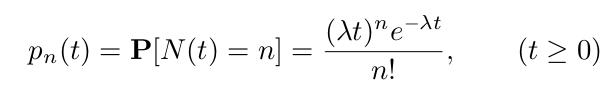
\includegraphics[scale=0.4]{im1}
\end{center}

for $n = 0, 1, 2, \ldots$ (remember $0! = 1$). It is assumed that $                                                                                                                                                                                                                                                                                                                                                                                                                                                                                                                                                                          N (t)$ can take the integer values $n = 0, 1, 2, \ldots$

\end{frame}
%%%%%%%%%%%%%%%%%%%%%%%%%%%%%%%%%%%%%%%%%%%%%%%%%%%%%%%%%%%%%%%%%%%%%%%%%%%%%%%%%%%%%%%%%%%%%%%%%%%%%%%%%%%%%
\begin{frame}
\frametitle{The Poisson process}
We can confirm that the previuos equation is a probability distribution by observing that

\begin{center}
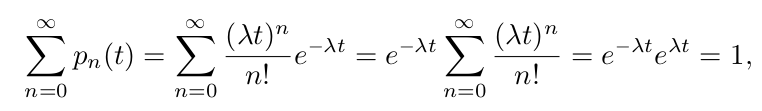
\includegraphics[scale=0.4]{im2}
\end{center}

Note that $p_{0}(0) = 1$, that is, the initial population size is 1.

\end{frame}

%%%%%%%%%%%%%%%%%%%%%%%%%%%%%%%%%%%%%%%%%%%%%%%%%%%%%%%%%%%%%%%%%%%%%%%%%%%%%%%%%%%%%%%%%%%%%%%%%%%%%%%%%%%%%
\begin{frame}
\frametitle{The Poisson process}
In fact, $p_{n}(t)$ is a Poisson probability (mass) function with parameter or intensity $\lambda$. For this reason any application for which Eqn holds is known as a Poisson process.
\begin{center}
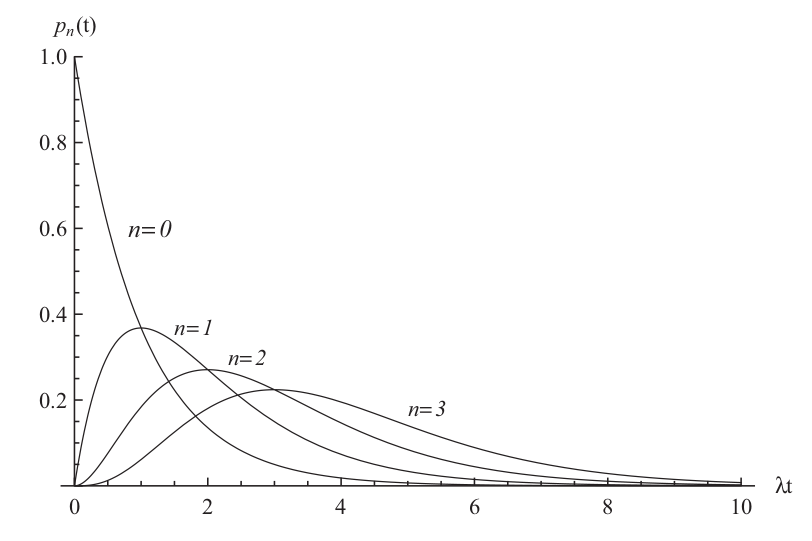
\includegraphics[scale=0.3]{im4}
\end{center}
\end{frame}


%%%%%%%%%%%%%%%%%%%%%%%%%%%%%%%%%%%%%%%%%%%%%%%%%%%%%%%%%%%%%%%%%%%%%%%%%%%%%%%%%%%%%%%%%%%%%%%%%%%%%%%%%%%%%
\begin{frame}
\frametitle{The Poisson process}
Since, for $n \geq 1$

\begin{center}
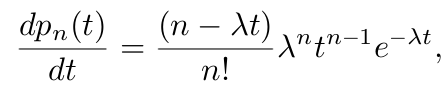
\includegraphics[scale=0.4]{im5}
\end{center}

The maximum values of the probabilities for fixed $n$ occur at time $t = n/\lambda$, where $dp_{n} (t)/dt = 0$. For $n = 0$.

\begin{center}
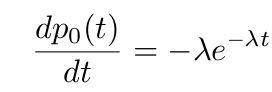
\includegraphics[scale=0.4]{im6}
\end{center}
\end{frame}
%%%%%%%%%%%%%%%%%%%%%%%%%%%%%%%%%%%%%%%%%%%%%%%%%%%%%%%%%%%%%%%%%%%%%%%%%%%%%%%%%%%%%%%%%%%%%%%%%%%%%%%%%%%%%
\begin{frame}
\frametitle{The Poisson process}
The mean $\mu (t)$ of the Poisson distribution is given by


\begin{center}
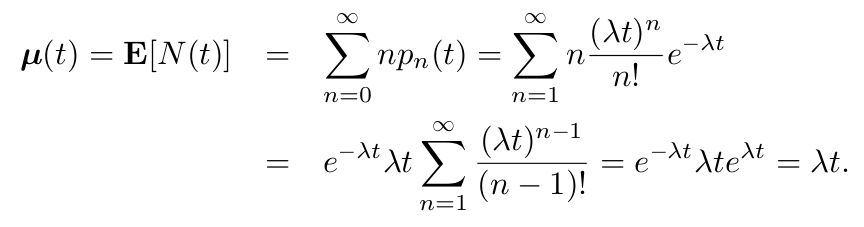
\includegraphics[scale=0.38]{im7}
\end{center}
Note that the mean value increases linearly with time at rate $\lambda$
   \end{frame}
%%%%%%%%%%%%%%%%%%%%%%%%%%%%%%%%%%%%%%%%%%%%%%%%%%%%%%%%%%%%%%%%%%%%%%%%%%%%%%%%%%%%%%%%%%%%%%%%%%%%%%%%%%%%%
\begin{frame}
\frametitle{The Poisson process}
Expressing the variance in terms of means, the variance is given by

\begin{center}
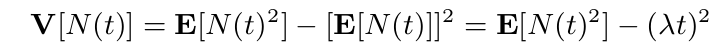
\includegraphics[scale=0.34]{im10}
\end{center}

Also

\begin{center}
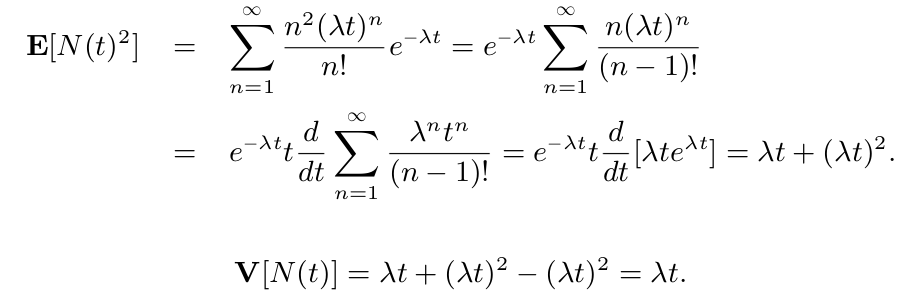
\includegraphics[scale=0.32]{im8}
\end{center}

Note that the Poisson distribution has the property that its mean is the same as its variance.
\end{frame}
%%%%%%%%%%%%%%%%%%%%%%%%%%%%%%%%%%%%%%%%%%%%%%%%%%%%%%%%%%%%%%%%%%%%%%%%%%%%%%%%%%%%%%%%%%%%%%%%%%%%%%%%%%%%%
\begin{frame}
\frametitle{Probabilidades de transición}
From
\begin{center}
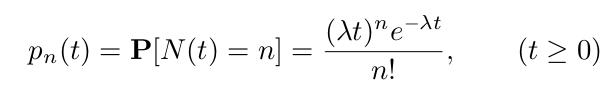
\includegraphics[scale=0.28]{im1}
\end{center}

\begin{center}
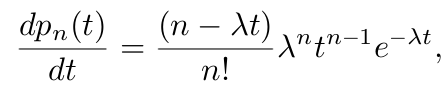
\includegraphics[scale=0.28]{im5}
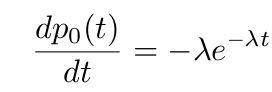
\includegraphics[scale=0.28]{im6}
\end{center}
given 
\begin{center}
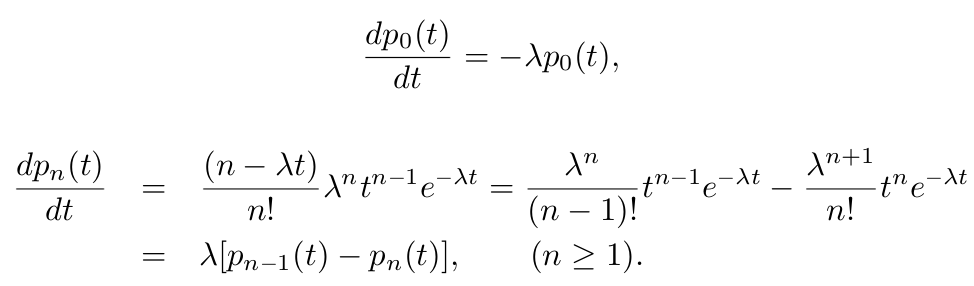
\includegraphics[scale=0.32]{im11}
\end{center}

\end{frame}
%%%%%%%%%%%%%%%%%%%%%%%%%%%%%%%%%%%%%%%%%%%%%%%%%%%%%%%%%%%%%%%%%%%%%%%%%%%%%%%%%%%%%%%%%%%%%%%%%%%%%%%%%%%%%
\begin{frame}
\frametitle{Probabilidades de transición}
These are differential-difference equations for the sequence of probabilities $p_{n}(t)$. From the definition of differentiation, the derivatives are obtained by the limiting process

\begin{center}
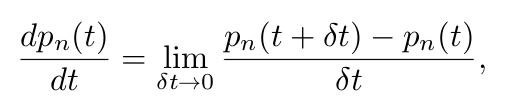
\includegraphics[scale=0.4]{im12}
\end{center}
so that approximately, for small $\delta t > 0$,

\begin{center}
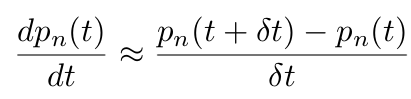
\includegraphics[scale=0.4]{im13}
\end{center}

\end{frame}
%%%%%%%%%%%%%%%%%%%%%%%%%%%%%%%%%%%%%%%%%%%%%%%%%%%%%%%%%%%%%%%%%%%%%%%%%%%%%%%%%%%%%%%%%%%%%%%%%%%%%%%%%%%%%
\begin{frame}
\frametitle{Probabilidad estacionaria o absoluta}
we can replace the equations by

\begin{center}
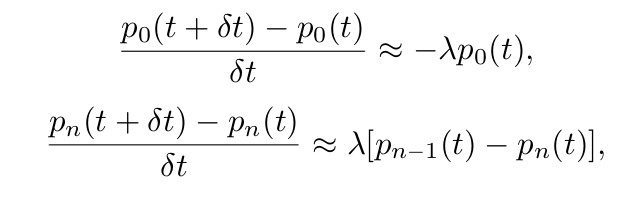
\includegraphics[scale=0.4]{im14}
\end{center}

so that

\begin{center}
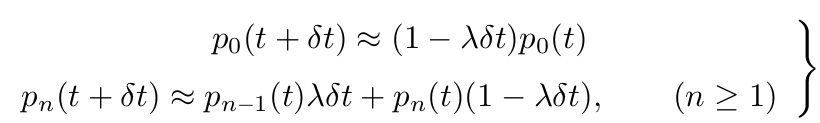
\includegraphics[scale=0.4]{im15}
\end{center}

\end{frame}

%%%%%%%%%%%%%%%%%%%%%%%%%%%%%%%%%%%%%%%%%%%%%%%%%%%%%%%%%%%%%%%%%%%%%%%%%%%%%%%%%%%%%%%%%%%%%%%%%%%%%%%%%%%%%
\begin{frame}
\frametitle{Probabilidad estacionaria o absoluta}

We can interpret the equations as follows. For the Geiger counter, we can infer from these formulas that the probability that a particle is recorded in the short time interval $\delta t$ is $ \lambda \delta t$, and that the probability that two or more particles are recorded is negligible, and consequently that no recording takes place with probability $(1 - \lambda \delta t)$. The only way in which the outcome reading $n(\geq 1)$ can occur at time $t + \delta t$ is that either one particle was recorded in the interval $\delta t$ when $n$ particles were
recorded at time $t$, or that nothing occurred with probability $(1 - \lambda \delta)$ when $n-1$ particles were recorded at time $t$.
\end{frame}

%%%%%%%%%%%%%%%%%%%%%%%%%%%%%%%%%%%%%%%%%%%%%%%%%%%%%%%%%%%%%%%%%%%%%%%%%%%%%%%%%%%%%%%%%%%%%%%%%%%%%%%%%%%%%

\end {document}



                                                  






